%!TEX root = ../TTK4550-MHT.tex
\section{Results}
\label{sec:results}

\subsection{Testing scheme}
The evaluation of the \gls{mht} algorithm is two-sided. Firstly the algorithm must be able to track under challenging conditions, and secondly it must be able to do so without having an ever growing computational cost and run time. The first performance metric is how well the algorithm is estimating the true position to the object it is tracking. We measure this by means of the Euclidean distance between the estimated and true track (\ref{eq:euclidian_distance_vector}).
\begin{equation}
	\Delta P = \| \V{p}_{track}-\V{p}_{target} \|_2
\label{eq:euclidian_distance_vector}
\end{equation}
The track is considered correct if $\Delta P \leq \varepsilon_p$ for all t after initial convergence. If a track is deviating more than the threshold and never return within the threshold again, it is considered lost at the time-step when it exceeded the threshold. If the track should converge after exceeding the threshold, it is considered restored at the time-step it is returning within the limit. 

The algorithm is tested on six scenarios:
\begin{itemize}
	\item Five fully cooperating ships
    \item Five partially cooperative ships
    \item Five ships avoiding obstacles with large space
    \item Five ships avoiding obstacles with little space
	\item Five almost parallel ships (normal speed \gls{radar})
	\item Five almost parallel ships (high speed \gls{radar})
\end{itemize}
\begin{figure}[H]
    \centering
    \begin{subfigure}{0.45\textwidth}
        \centering
        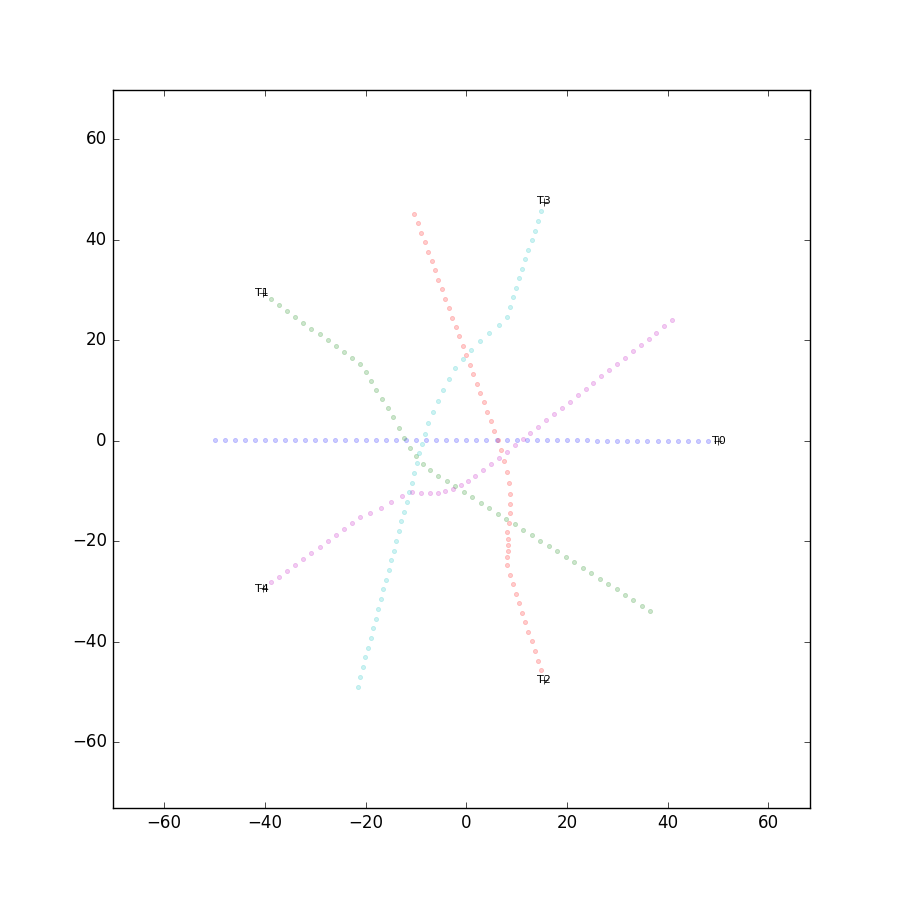
\includegraphics[height=0.27\textheight]{scenario1}
        \caption{First scenario}
    \end{subfigure}
    \begin{subfigure}{0.45\textwidth}
        \centering
        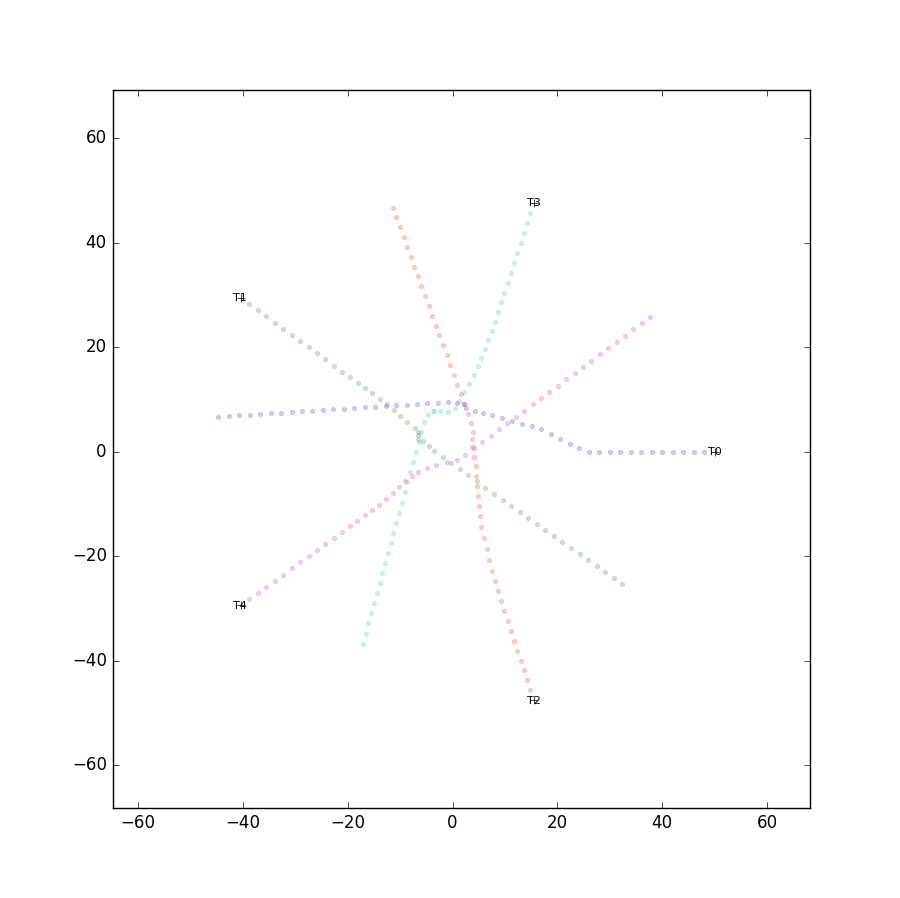
\includegraphics[height=0.27\textheight]{scenario2}
        \caption{Second scenario}
    \end{subfigure}
    \begin{subfigure}{0.45\textwidth}
        \centering
        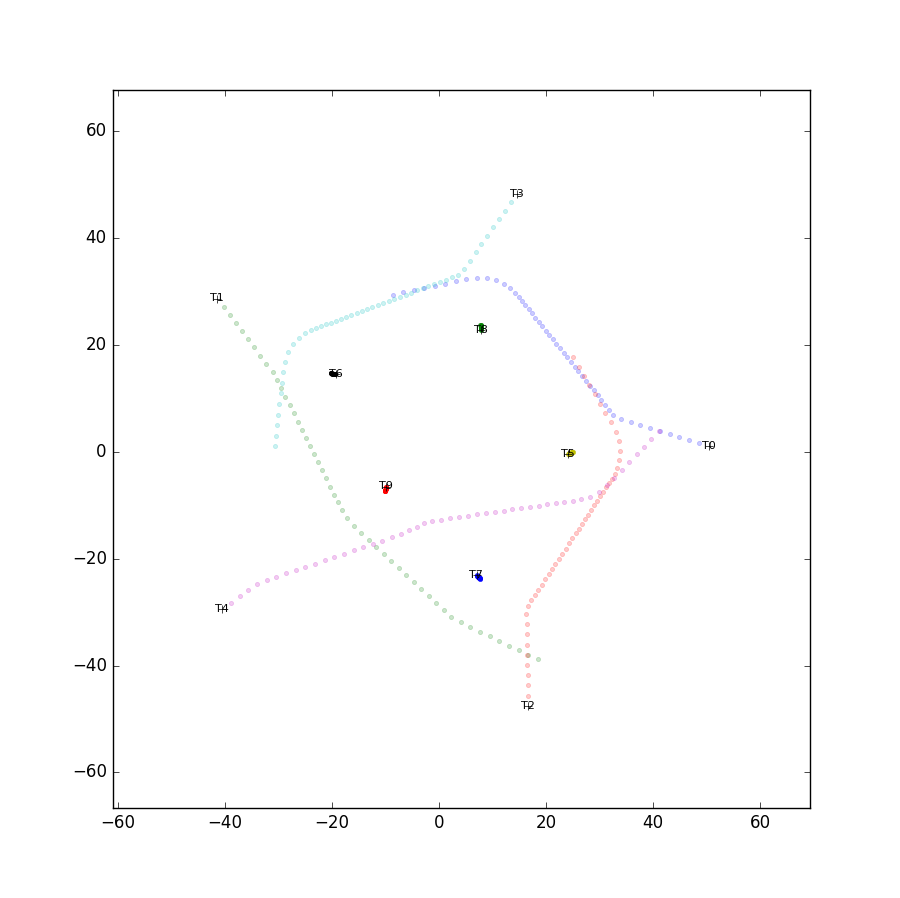
\includegraphics[height=0.27\textheight]{scenario3}
        \caption{Third scenario}
    \end{subfigure}
    \begin{subfigure}{0.45\textwidth}
        \centering
        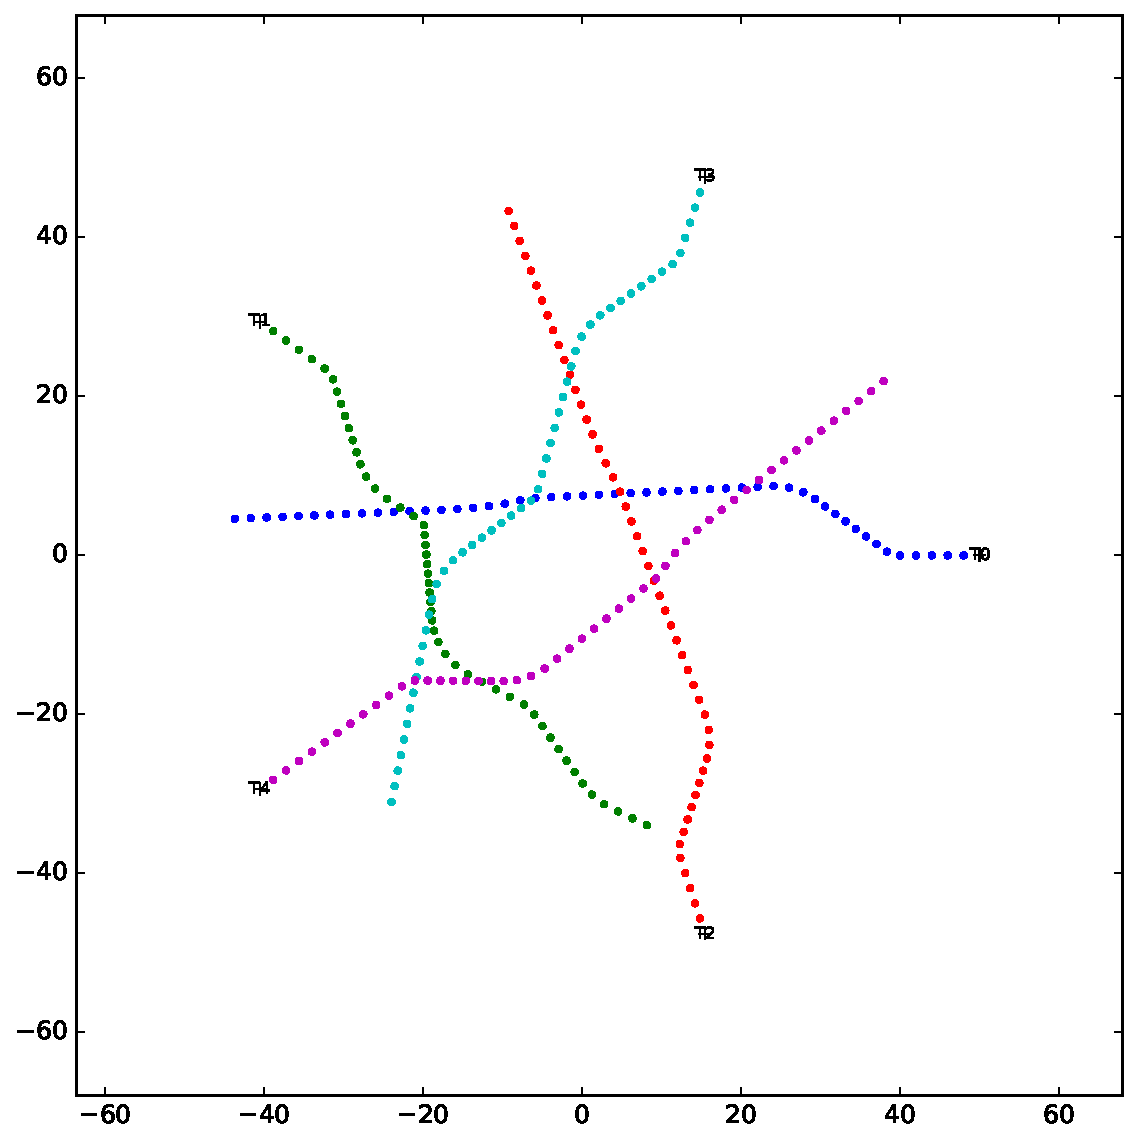
\includegraphics[height=0.27\textheight]{scenario4}
        \caption{Fourth scenario}
    \end{subfigure}
    \begin{subfigure}{0.45\textwidth}
        \centering
        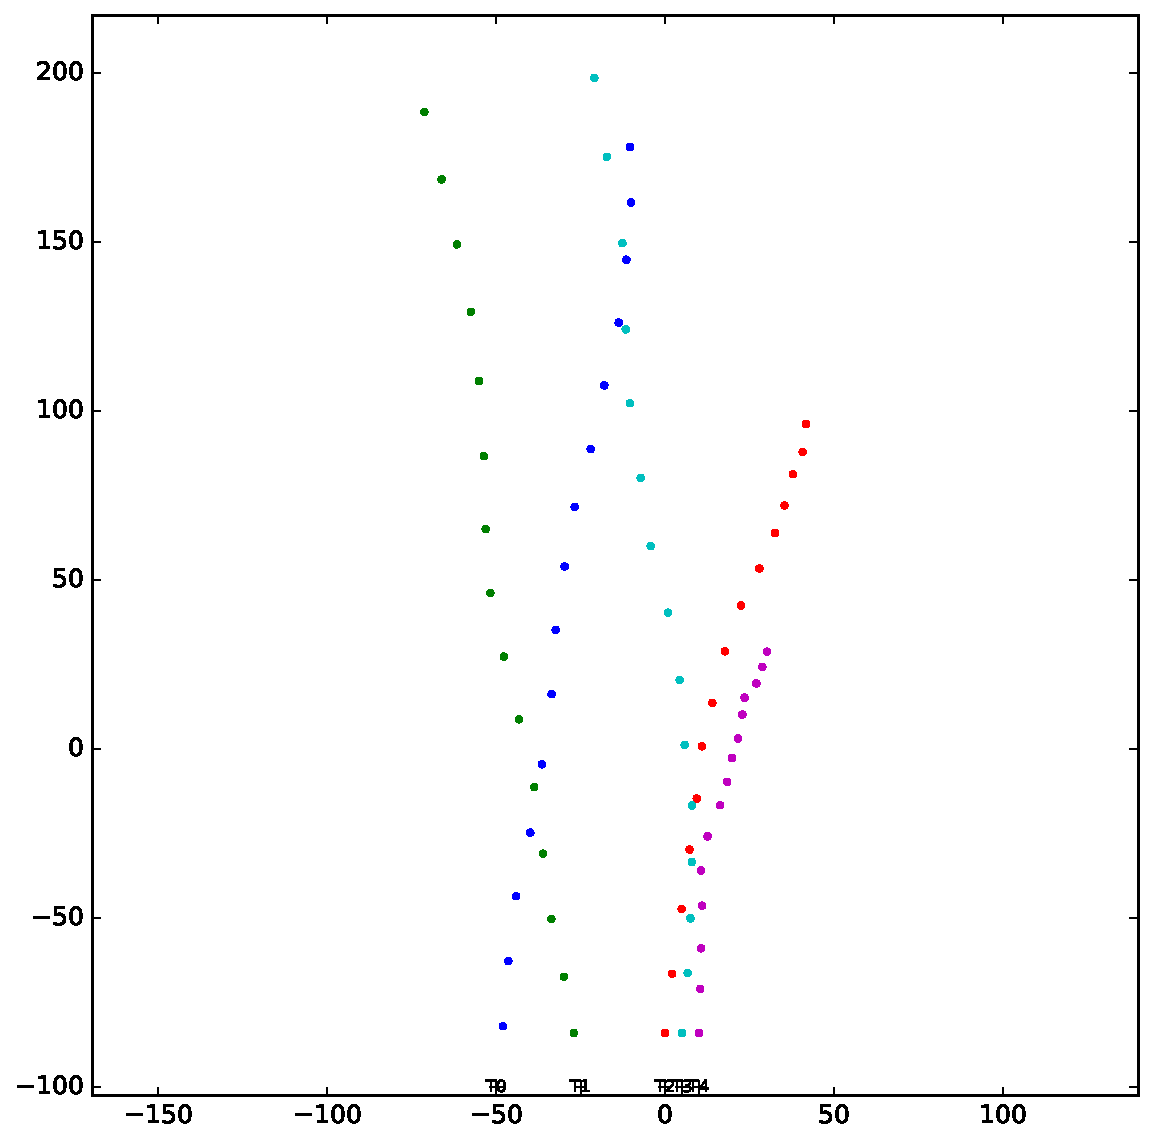
\includegraphics[height=0.27\textheight]{scenario5}
        \caption{Fifth scenario}
    \end{subfigure}
    \begin{subfigure}{0.45\textwidth}
        \centering
        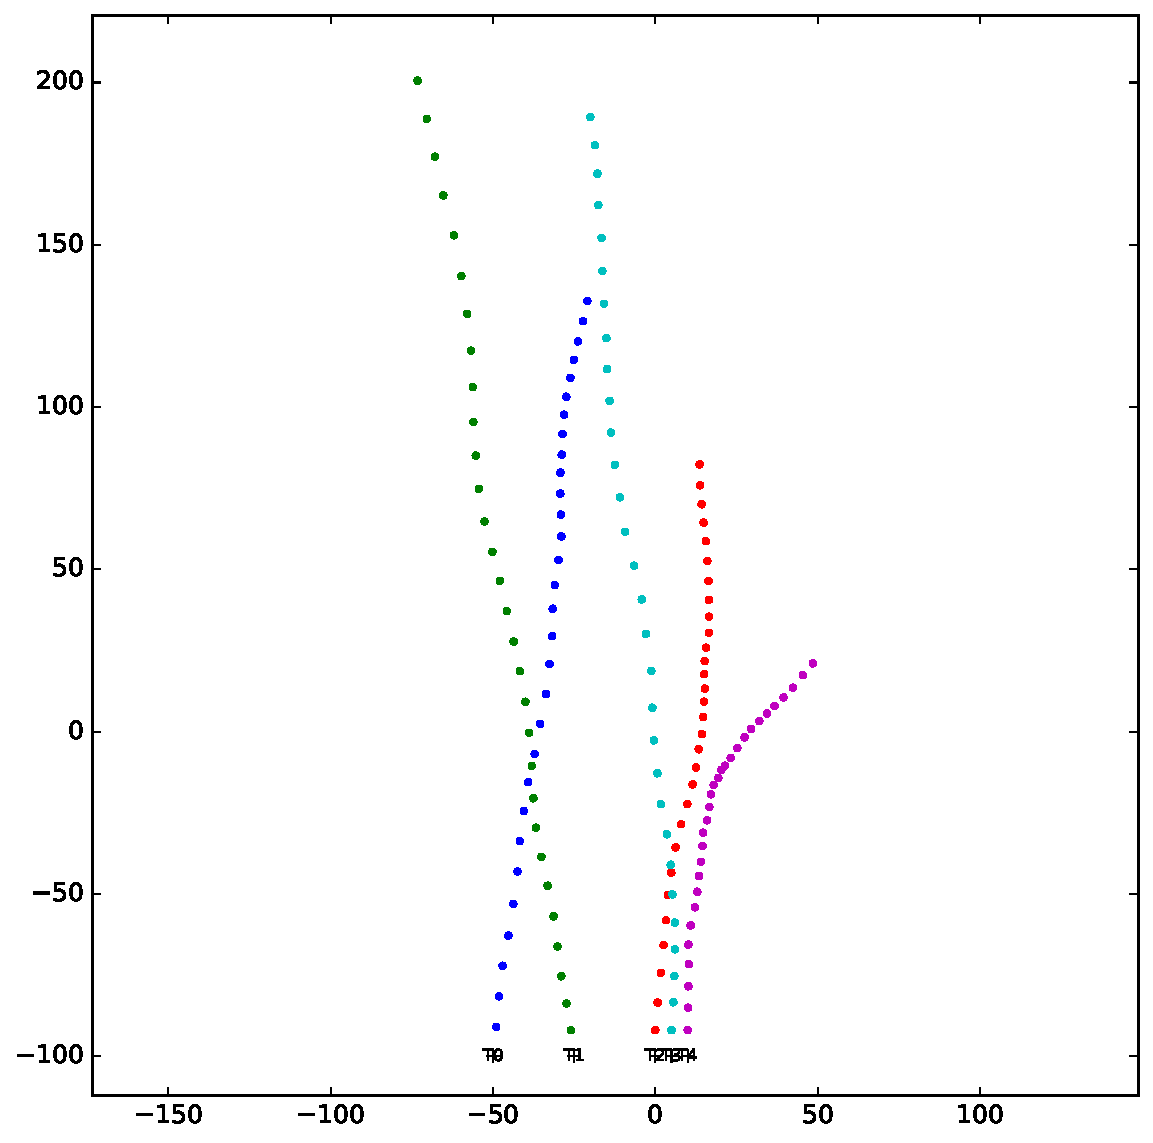
\includegraphics[height=0.27\textheight]{scenario6}
        \caption{Sixth scenario}
    \end{subfigure}
    \caption{True track for scenario 1-6}
    \label{fig:true_tracks}
\end{figure} 

\subsection{Simulation data}
Scenario one through four was generated as a recording of time and position from an \gls{asv} simulator with \gls{colav}, developed by Dr. D. Kwame Minde  Kufolaor at \gls{ntnu}. The ships are configured such that they need to maneuver to avoid collision with each other, which allows for tracking of maneuvering targets in close proximity to each other. These scenarios where sampled at 1 Hz which is a little faster than a normal high speed vessel \gls{radar} at 0.8 Hz (48 \gls{rpm}). The fifth and sixth scenario was generated as a part of this project, and is composed by linear parallel paths with white Gaussian system noise as maneuvering. These scenarios were sampled from the same data set at 0.5 Hz  and 1 Hz respectively, where 0.5 Hz is a little higher that a normal maritime coastal \gls{radar} at 0.4 Hz (24 \gls{rpm}). The usage of two different sample rates were to compare the most common \gls{radar} update frequencies used in the maritime sector with respect to tracking performance. The different ranges, \gls{fov}, and expected clutter points for the different scenarios are summarized in Table \ref{tab:clutter_measurements}.

\begin{table}
\centering
\begin{tabular}{c c c c c c c c}
			&				&						& & &$\lambda_\phi \cdot FOV$& 	&		\\
Scenario 	& Radar range	& \gls{fov}				& $1$ 	& $2$ 	& $4$ 	&$6$ 	& $8$	\\ \hline
1-4		 	& $65 m$ 		& $1.3\cdot10^4 m^2$	& 1.3 	& 2.6 	& 5.2 	& 7.38 	& 9.21 	\\
5-6		 	& $155 m$		& $7.5\cdot10^4 m^2$	& 3.22 	& 4.61 	& 5.99 	& 7.38 	& 9.21 					
\end{tabular}
\caption{Expected number of clutter measurements in scenarios}
\label{tab:clutter_measurements}
\end{table}

\subsection{Simulations}
Scenario one through six was simulated with the following variations with all four solvers.
\begin{equation*}
\begin{split}
\V{P_D} &= \begin{bmatrix} 0.5 & 0.6 & 0.7 & 0.8 & 0.9 \end{bmatrix} \\
\V{N} &=\begin{bmatrix} 0 & 1 & 3 & 6 & 9 \end{bmatrix} \\
\V{\lambda_\phi} &=\begin{bmatrix} 0 & 1\cdot10^{-4} & 2\cdot10^{-4} & 4\cdot10^{-4} & 6\cdot10^{-4} & 8\cdot10^{-4} \end{bmatrix}
\end{split}
\end{equation*}
Each of the 3600 variants was simulated 160 times with different seeded random clutter measurements and misdetections. These simulations required approximately 864 \gls{cpu} hours, and were for the most part simulated on a 36 core virtualized server. For each simulation, the estimated tracks were compared with the true tacks and categorised in successful and lost tracks, where the track loss threshold $\epsilon_p$ was $4$ meters. Figure \ref{fig:track_hypotheses_example} display a mid-simulation plot with current best tracks in solid lines, and hypotheses in dotted lines. Notice how many of the hypotheses have very similar paths, and with a certain margin duplicates each other.
\begin{figure}[H]
    \centering
    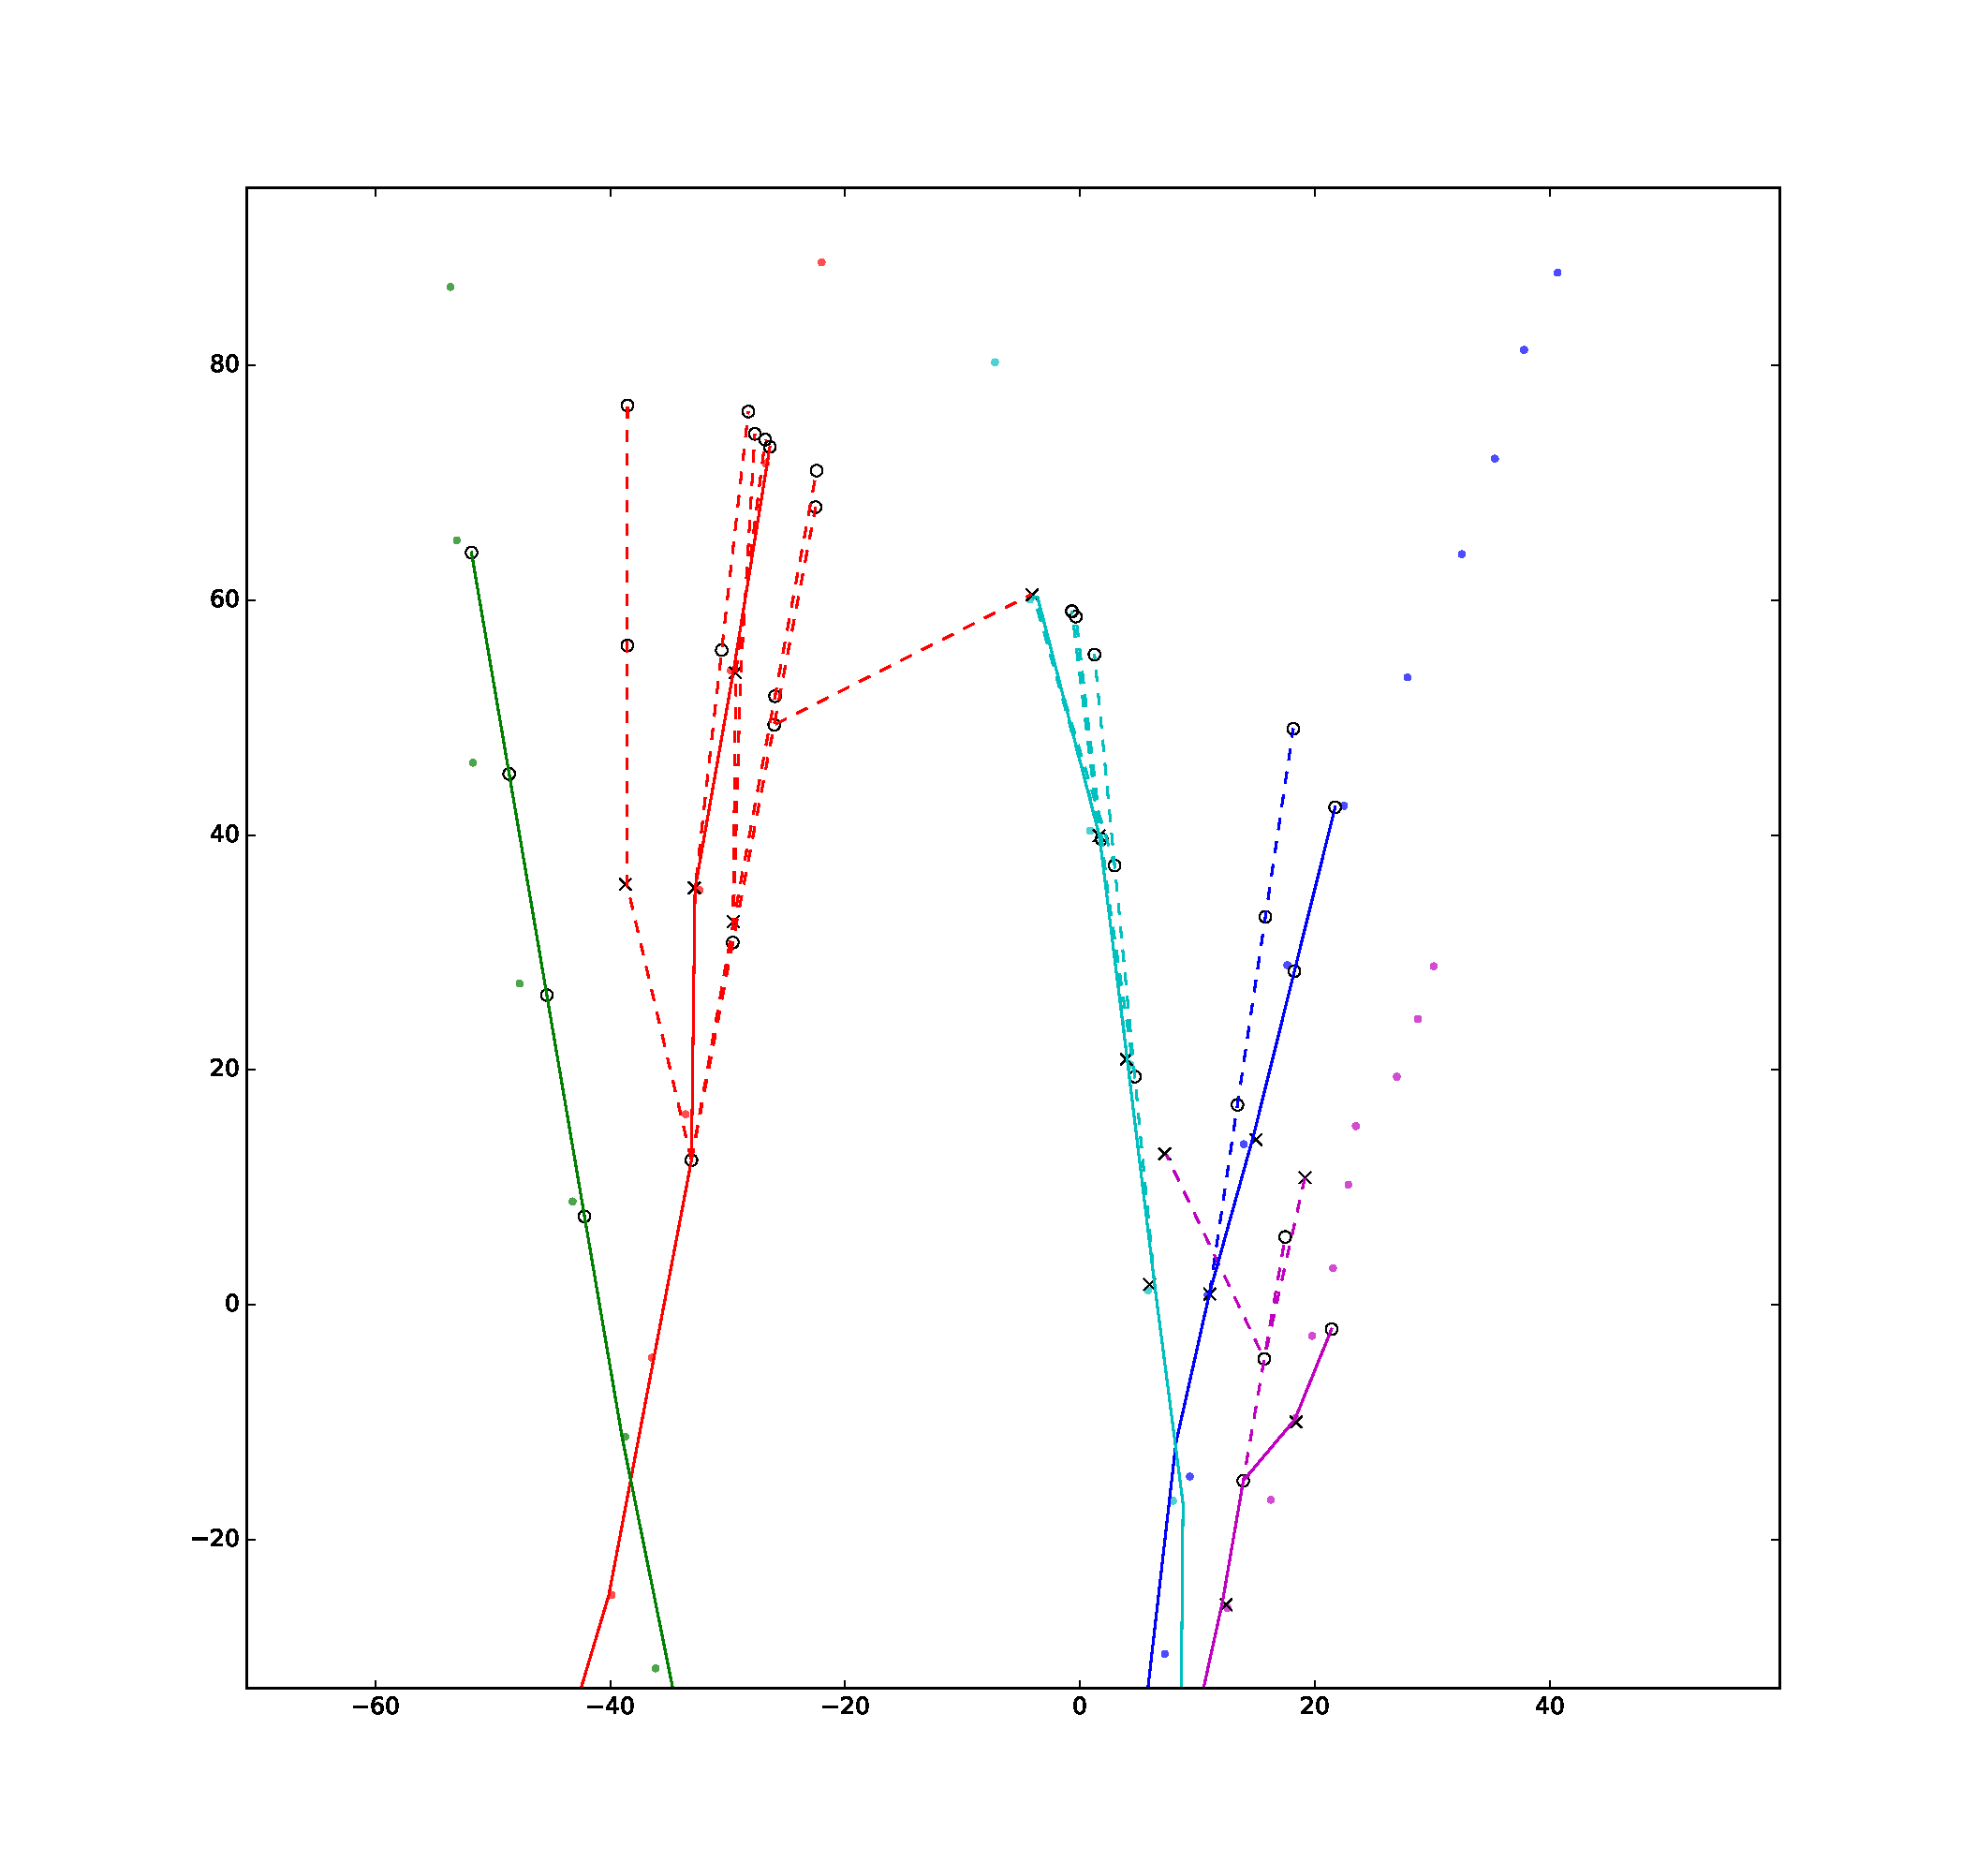
\includegraphics[clip, trim=3cm 2.5cm 3cm 3cm,width=0.7\textwidth]{tracks_with_hypotheses}
    \caption{Track hypotheses example}
    \label{fig:track_hypotheses_example}
\end{figure}
Figure \ref{fig:tracking_performance} shows the track performance from the "GLPK" solver. The performance of the other solvers can be found in the appendix, Figures \ref{fig:dynamic_agents_full_cooperation_cropped} - \ref{fig:dynamic_and_static_agents_narrow_space_cropped}.
\begin{figure}[H]
    \centering
    \begin{subfigure}{0.49\textwidth} 
        \centering
        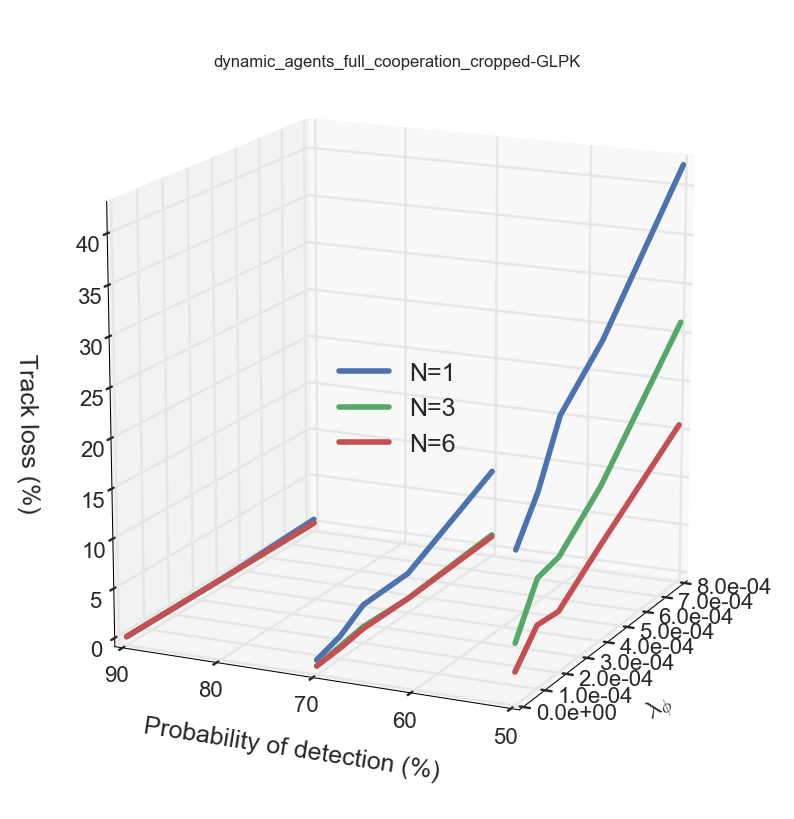
\includegraphics[clip, trim=0cm 1cm 0cm 1cm, height=0.28\textheight]{dynamic_agents_full_cooperation_cropped-GLPK}
        \caption{Scenario 1}
    \end{subfigure}
    \begin{subfigure}{0.49\textwidth}
        \centering
        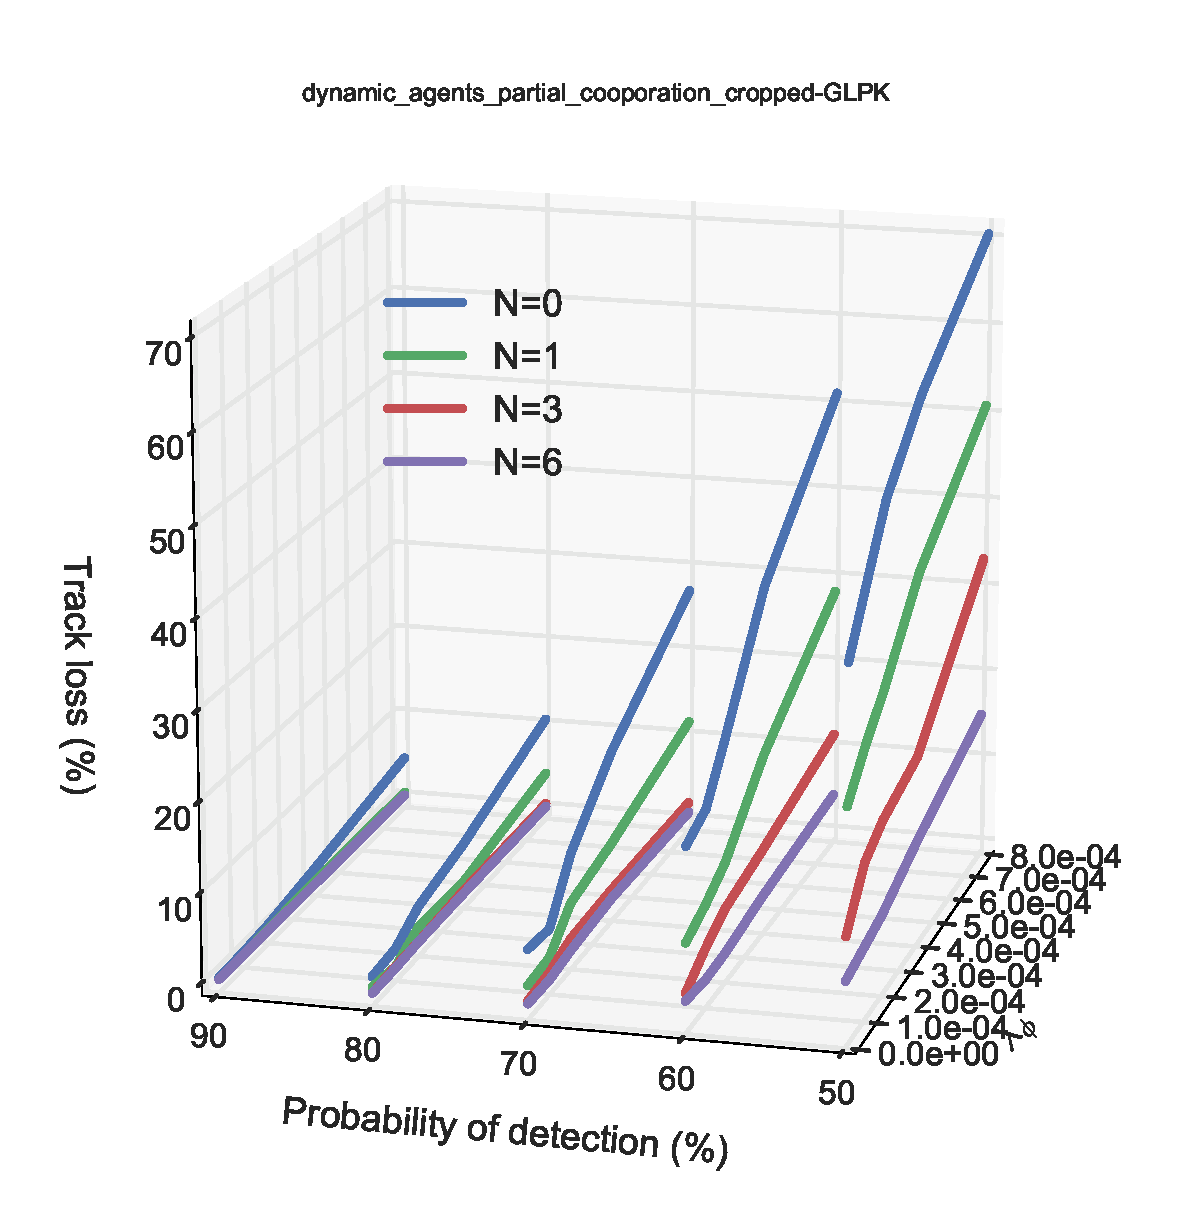
\includegraphics[clip,  trim=0cm 1cm 0cm 1cm,height=0.28\textheight]{dynamic_agents_partial_cooporation_cropped-GLPK}
        \caption{Scenario 2}
    \end{subfigure}
    \begin{subfigure}{0.49\textwidth}
        \centering
        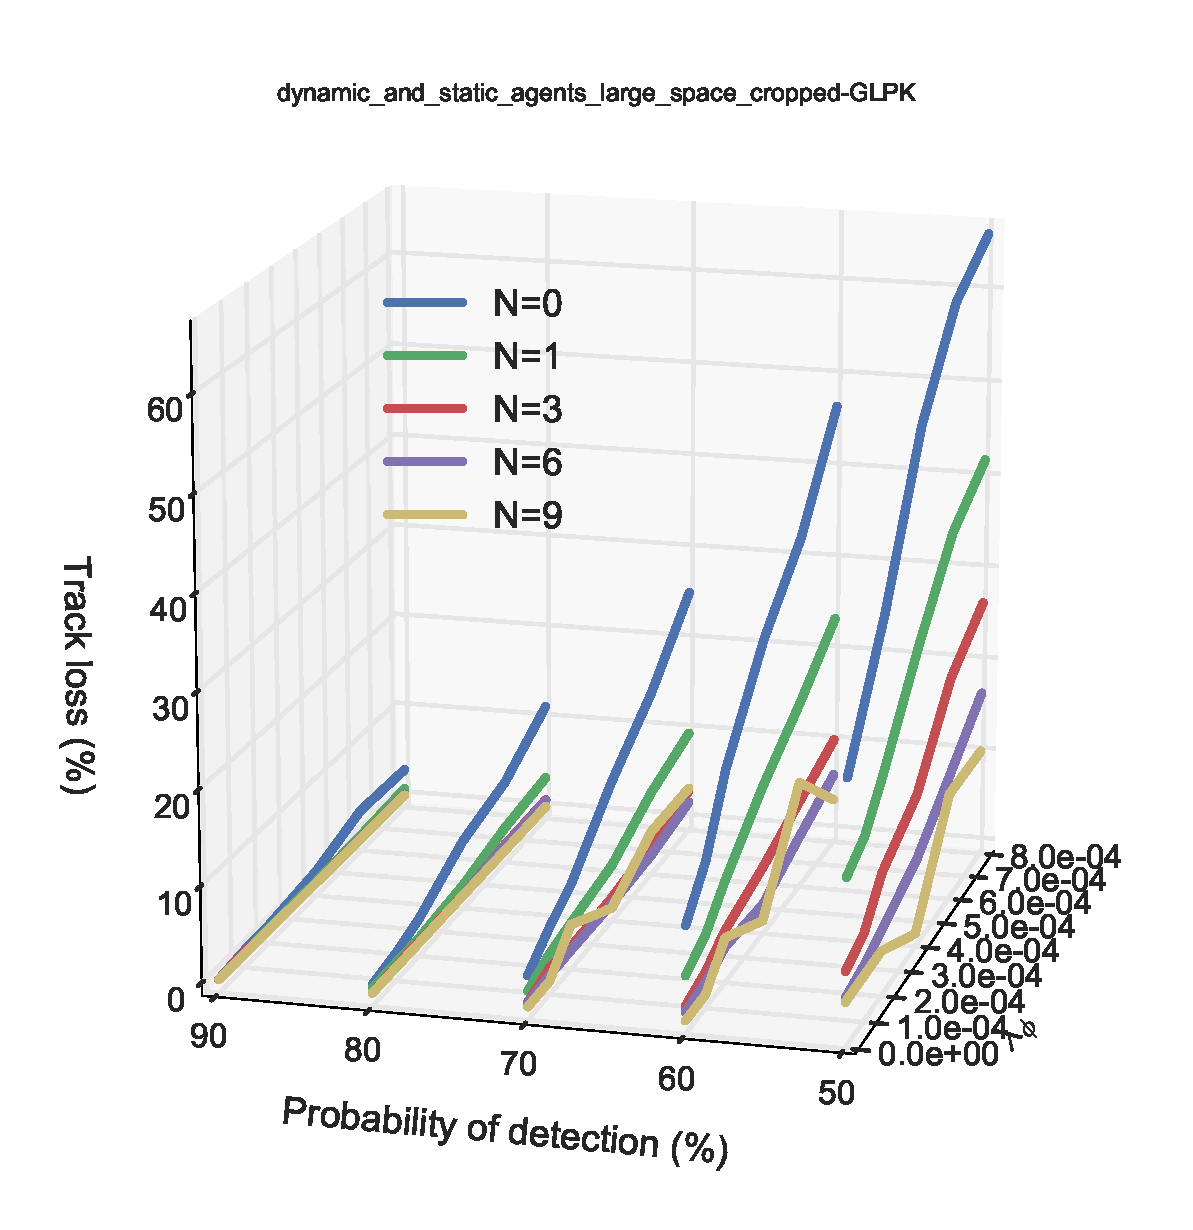
\includegraphics[clip,  trim=0cm 1cm 0cm 1cm,height=0.28\textheight]{dynamic_and_static_agents_large_space_cropped-GLPK}
        \caption{Scenario 3}
    \end{subfigure}
    \begin{subfigure}{0.49\textwidth}
        \centering
        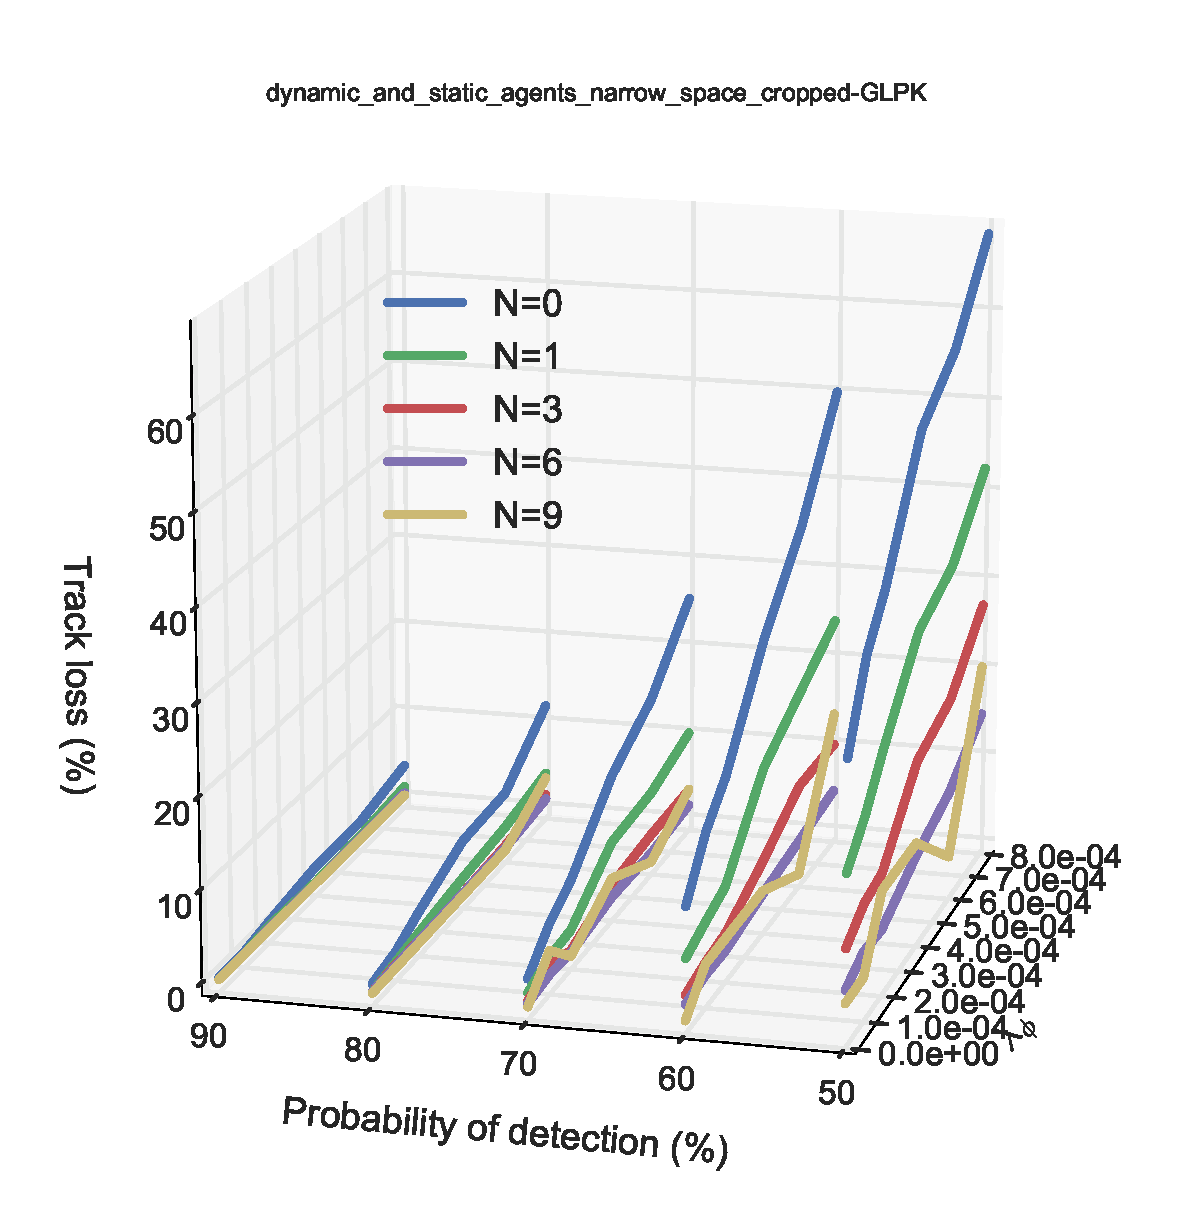
\includegraphics[clip,  trim=0cm 1cm 0cm 1cm,height=0.28\textheight]{dynamic_and_static_agents_narrow_space_cropped-GLPK}
        \caption{Scenario 4}
    \end{subfigure}
     \begin{subfigure}{0.49\textwidth}
        \centering
        \includegraphics[clip,  trim=0cm 1cm 0cm 1cm,height=0.28\textheight]{{parallel_targets_0.5hz-GLPK}.pdf}
        \caption{Scenario 5}
    \end{subfigure}
     \begin{subfigure}{0.49\textwidth}
        \centering
        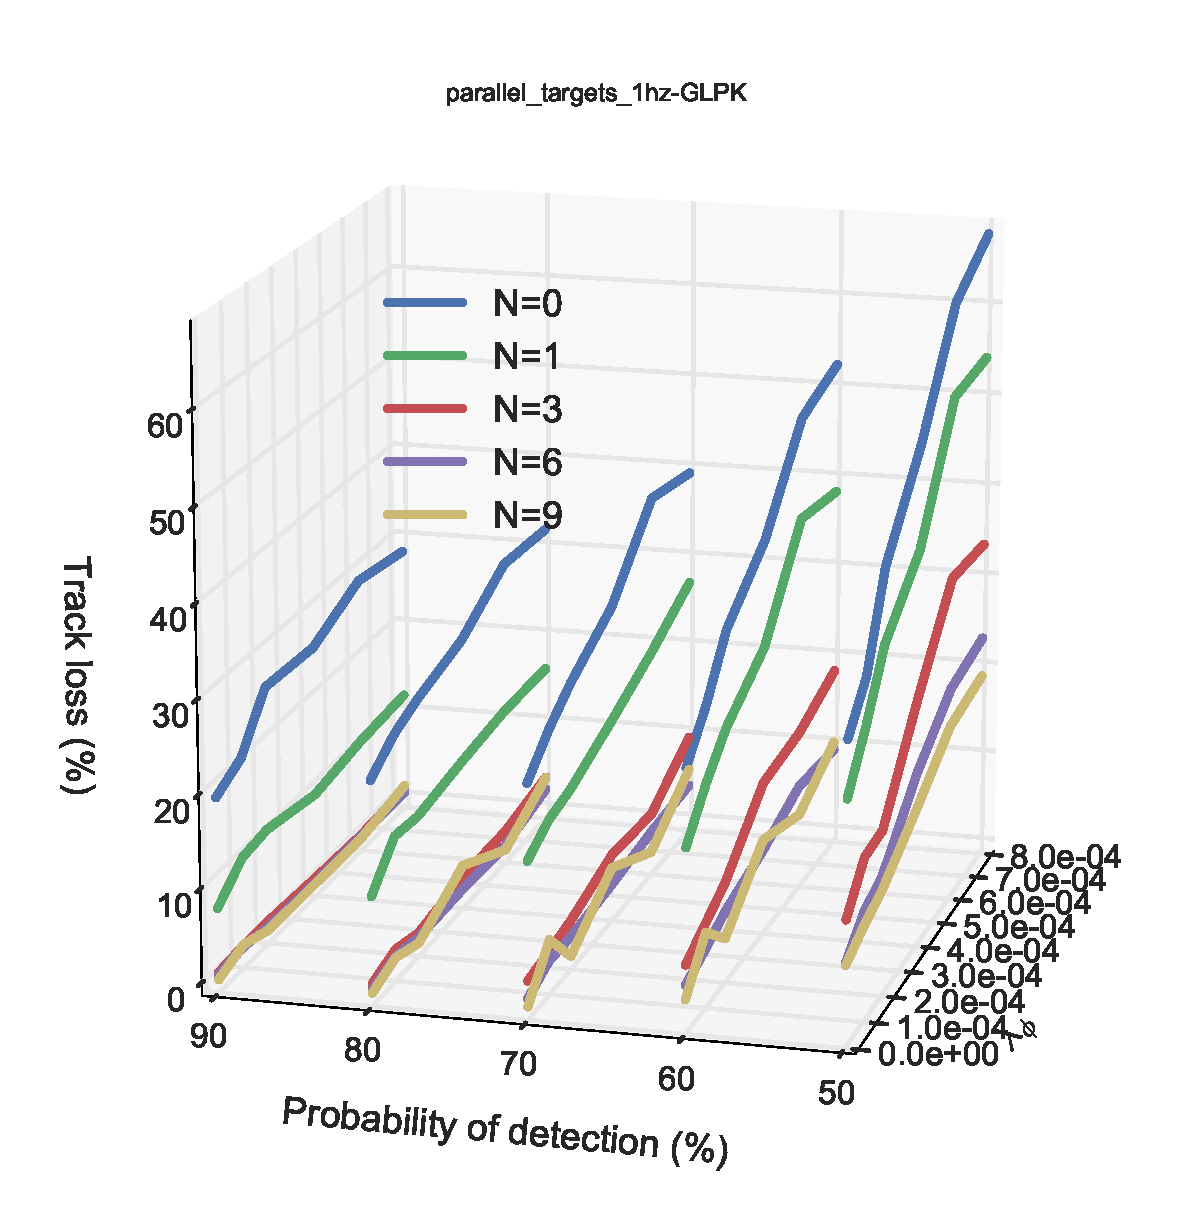
\includegraphics[clip,  trim=0cm 1cm 0cm 1cm,height=0.28\textheight]{parallel_targets_1hz-GLPK}
        \caption{Scenario 6}
    \end{subfigure}
	\caption{Simulation results for all scenarios}
    \label{fig:tracking_performance}
\end{figure}

\subsection{Runtime}
Figure \ref{fig:runtime_scenario_1} to \ref{fig:runtime_scenario_5} displays the average the runtime for the different solvers. The runtime along the z-axis displays the time used for simulating the entire scenario.

\begin{figure}[H]
\centering
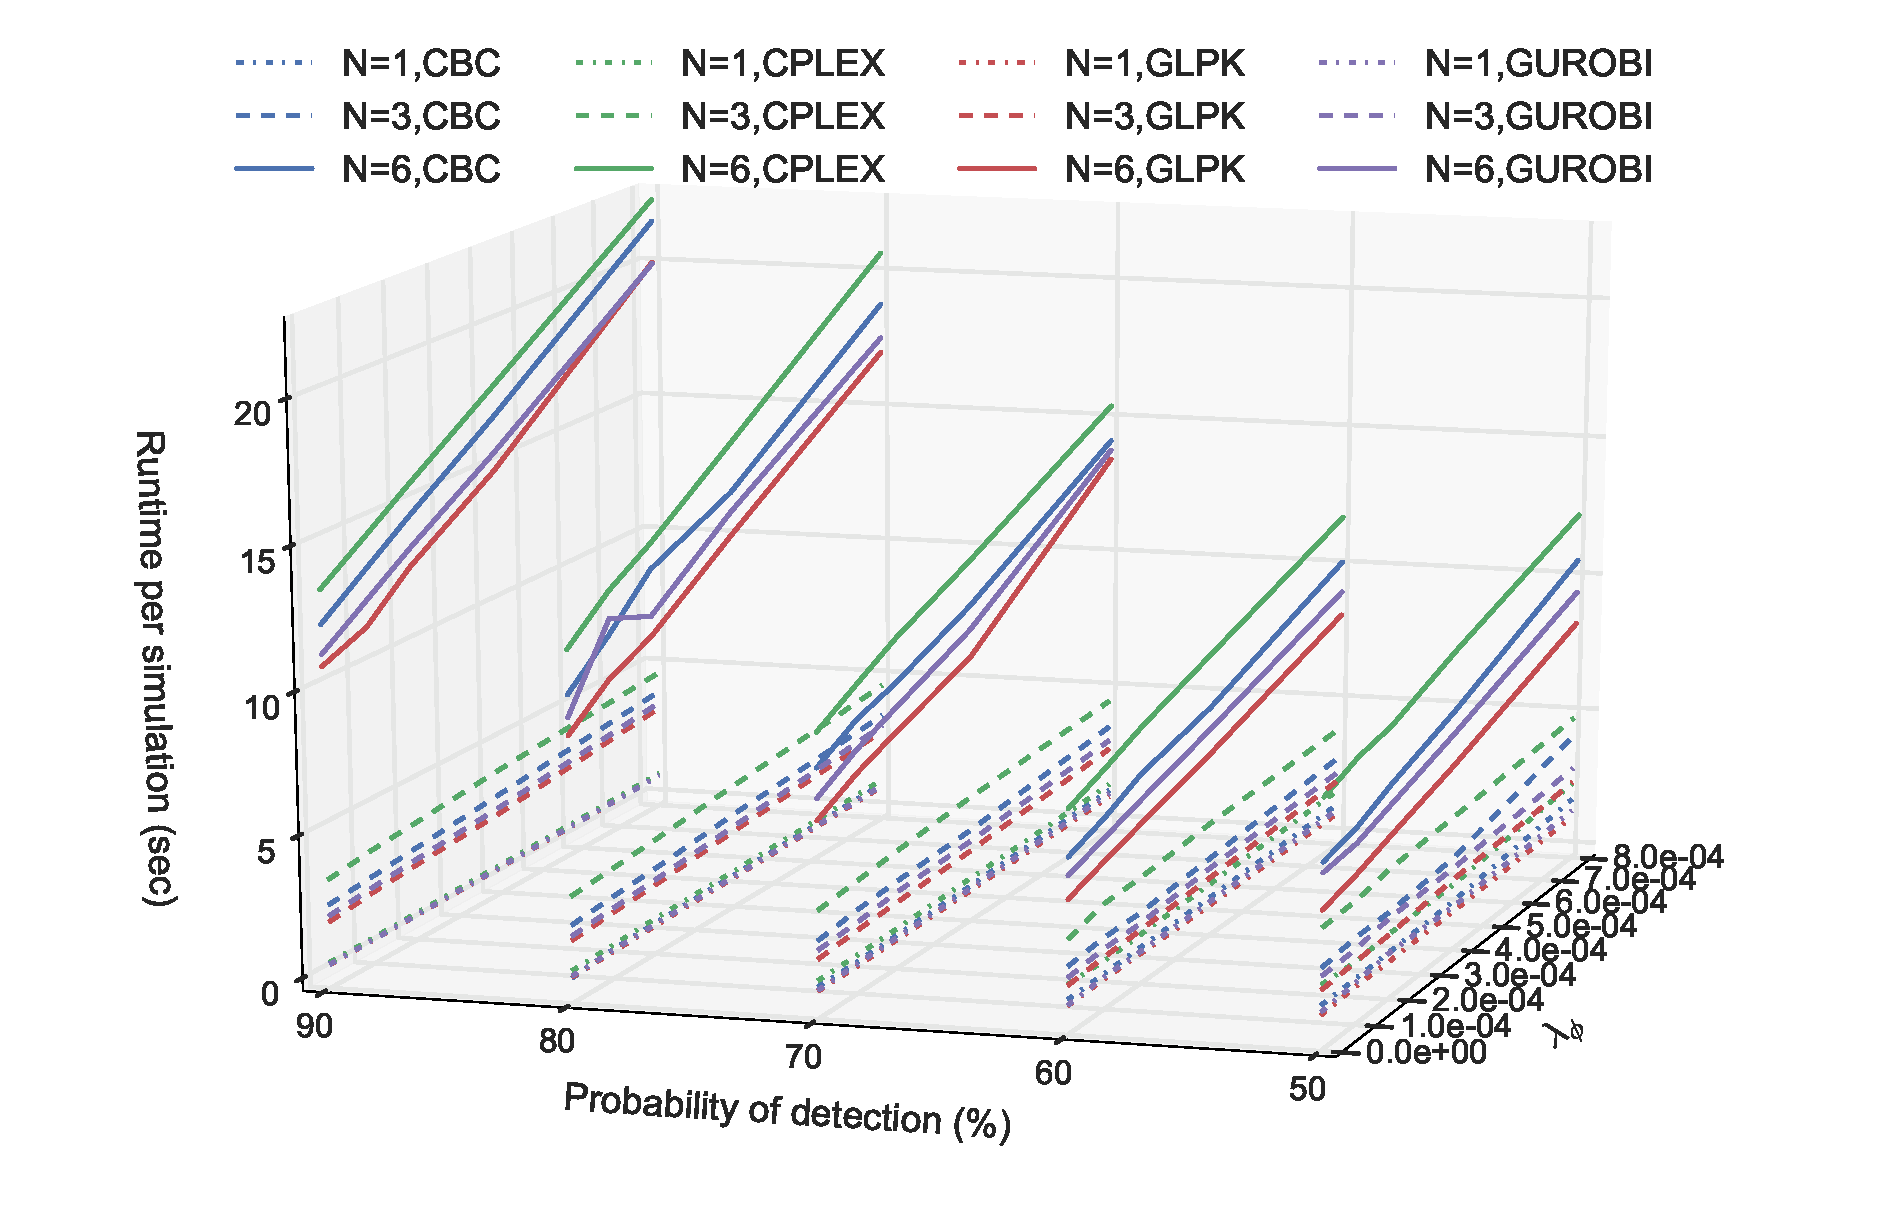
\includegraphics[clip, trim=0cm 1.5cm 0cm 0cm, width=\textwidth]{dynamic_agents_full_cooperation_cropped_runtime}
\caption{Runtime for scenario 1}
\label{fig:runtime_scenario_1}
\end{figure}

\begin{figure}[H]
\centering
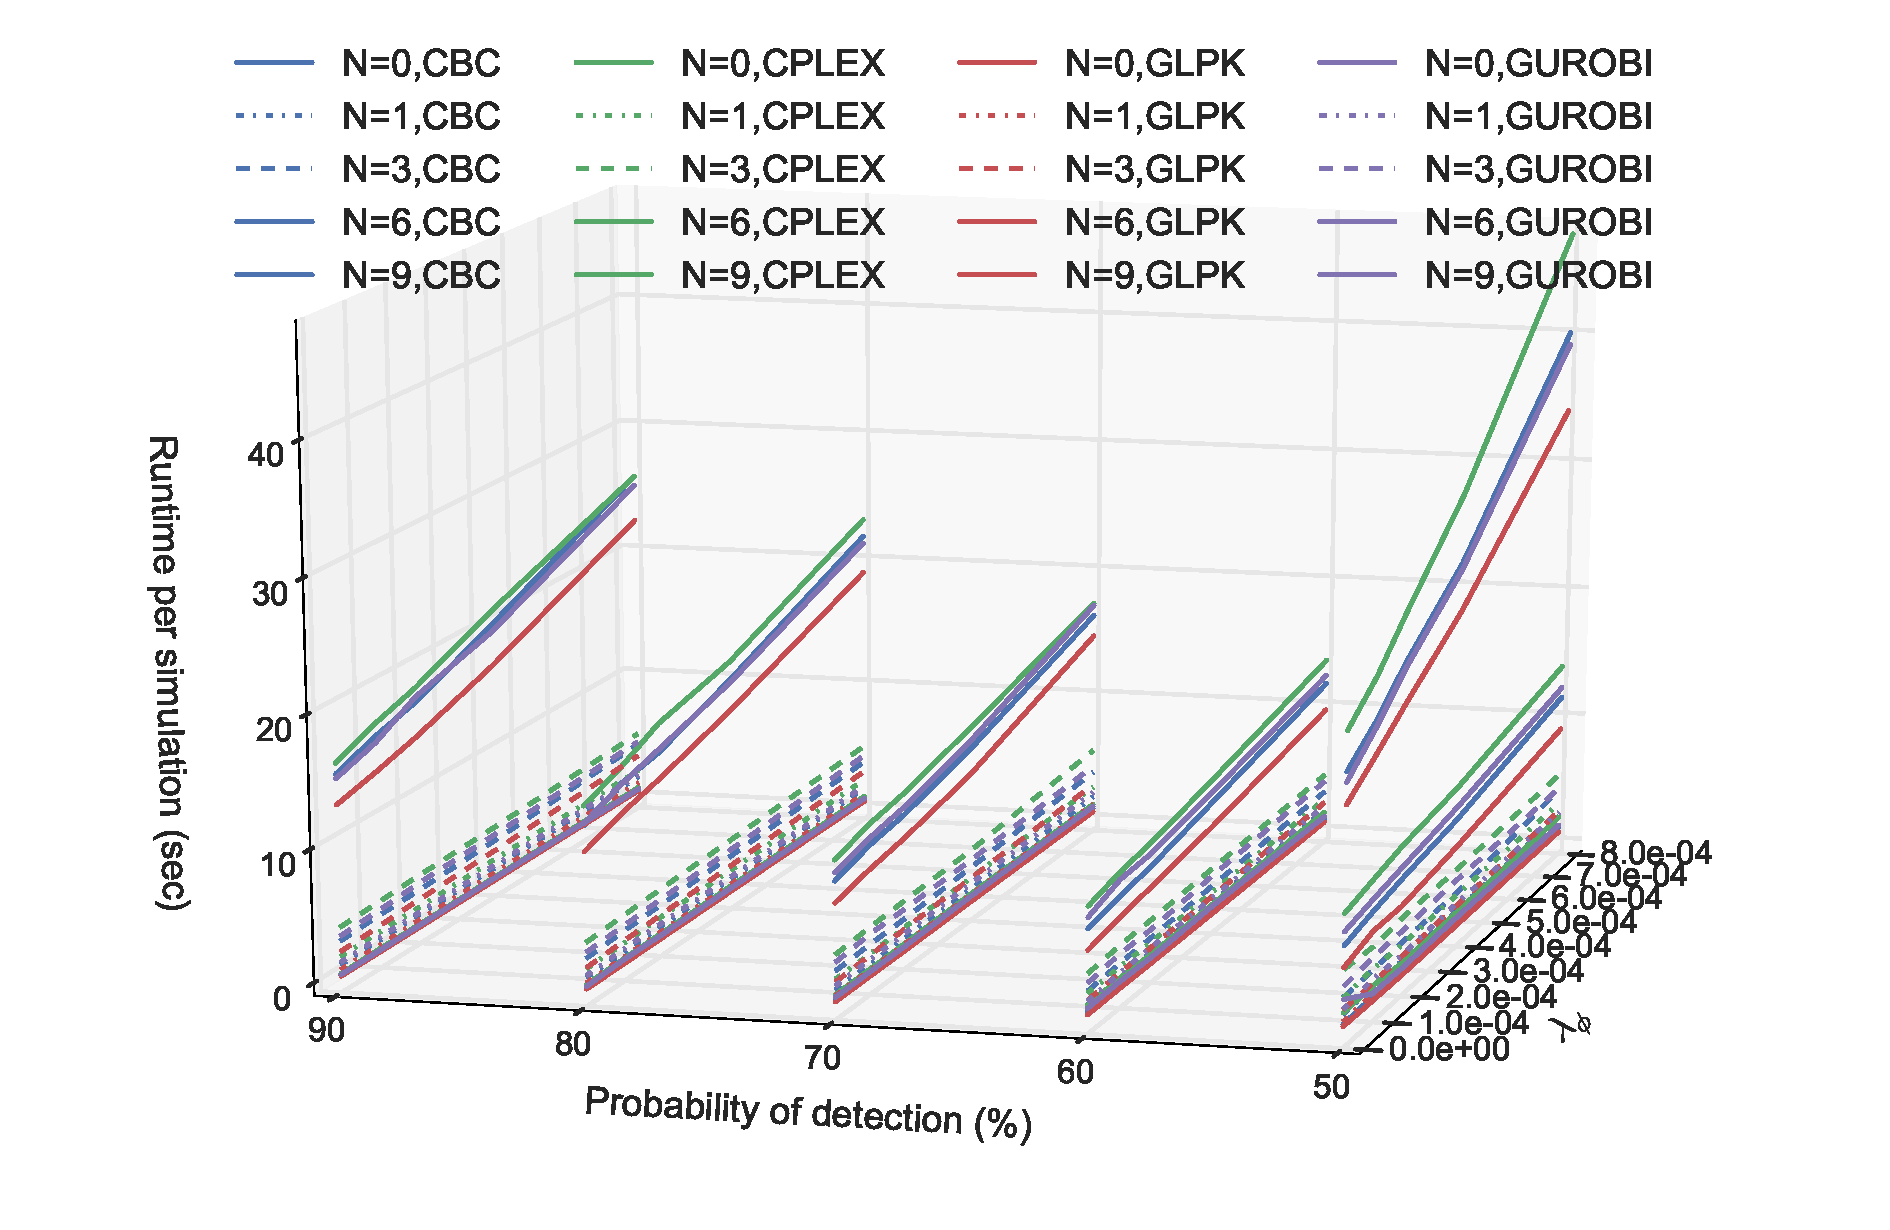
\includegraphics[clip, trim=0cm 1.5cm 0cm 0cm,width=\textwidth]{dynamic_agents_partial_cooporation_cropped_runtime}
\caption{Runtime for scenario 2}
\label{fig:runtime_scenario_2}
\end{figure}

\begin{figure}[H]
\centering
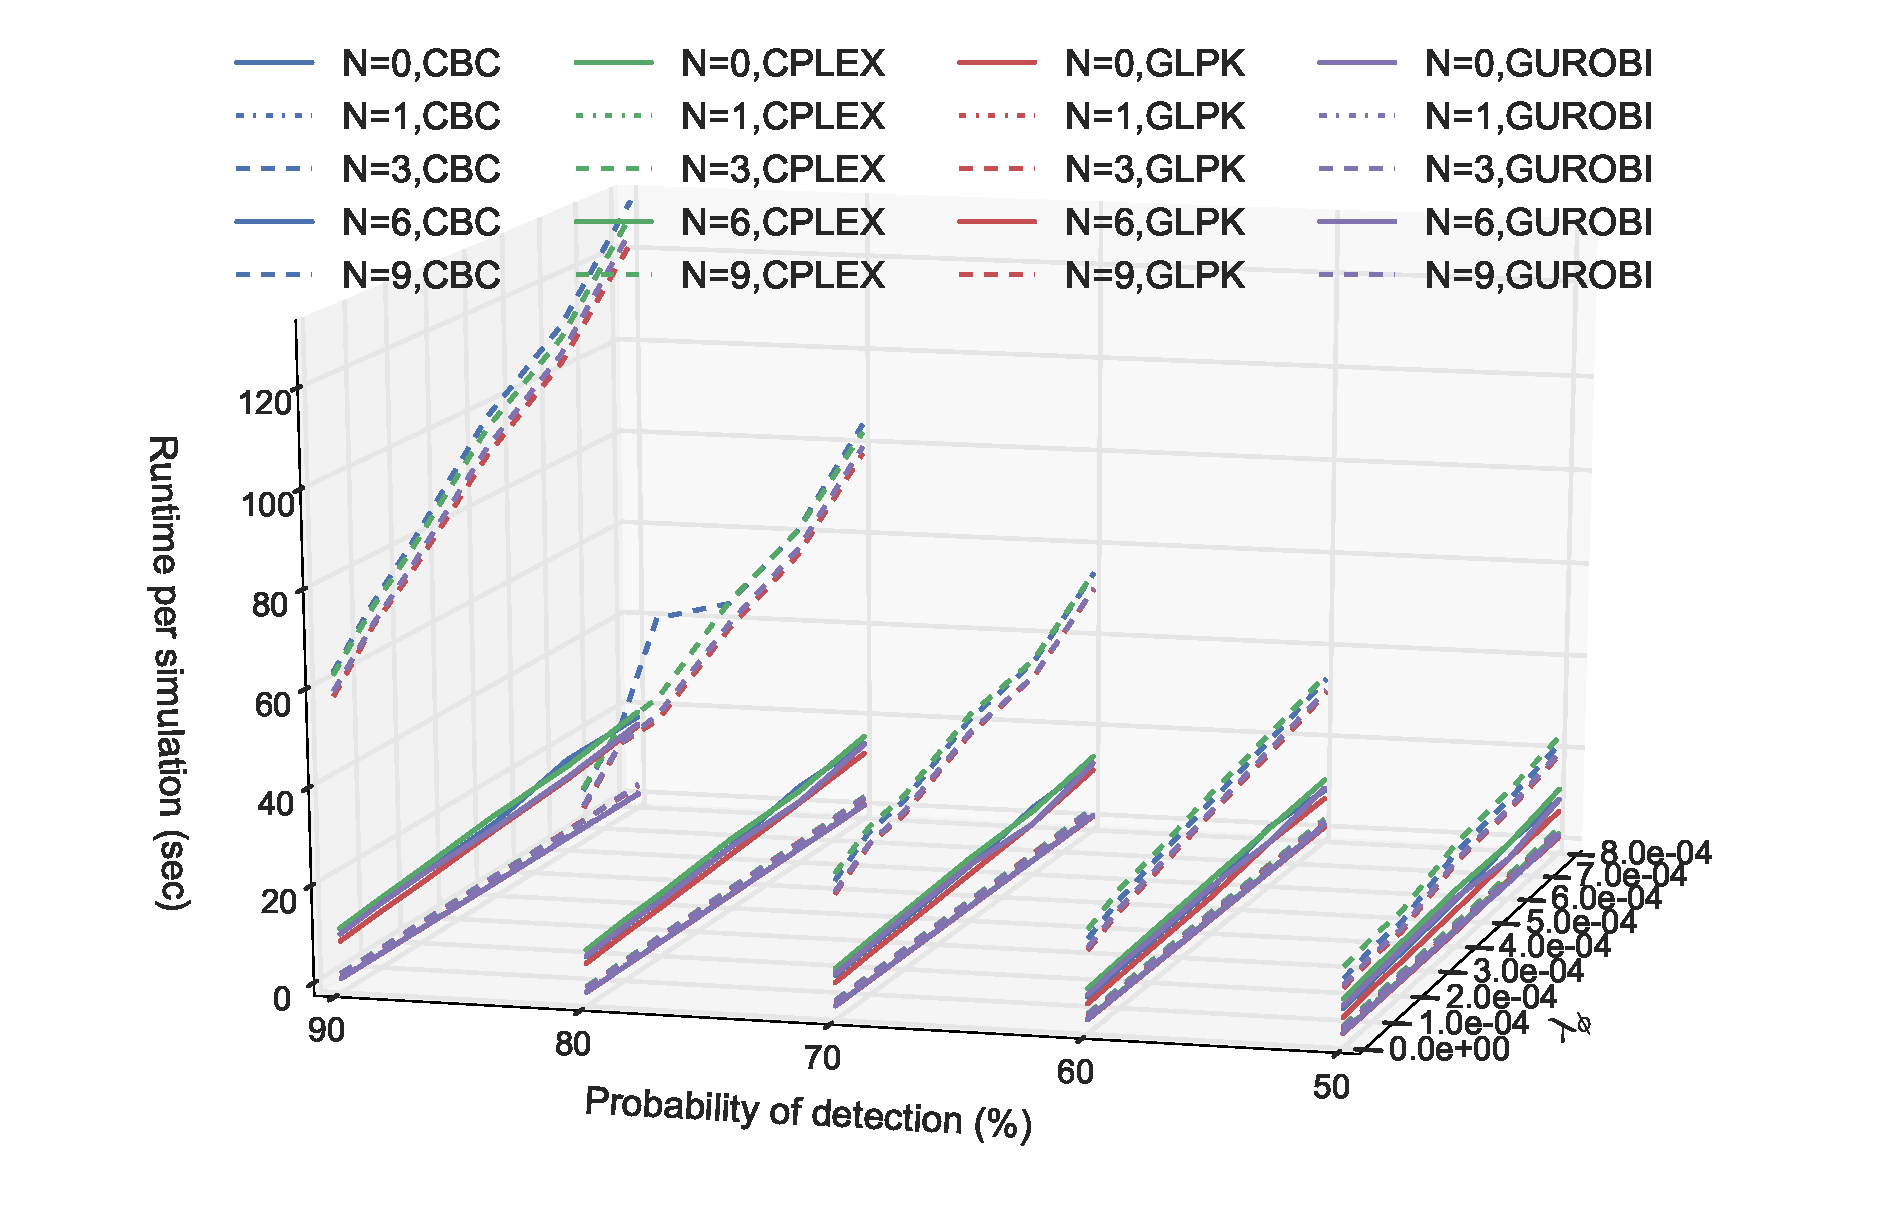
\includegraphics[clip, trim=0cm 1.5cm 0cm 0cm,width=\textwidth]{dynamic_and_static_agents_large_space_cropped_runtime}
\caption{Runtime for scenario 3}
\label{fig:runtime_scenario_3}
\end{figure}

\begin{figure}[H]
\centering
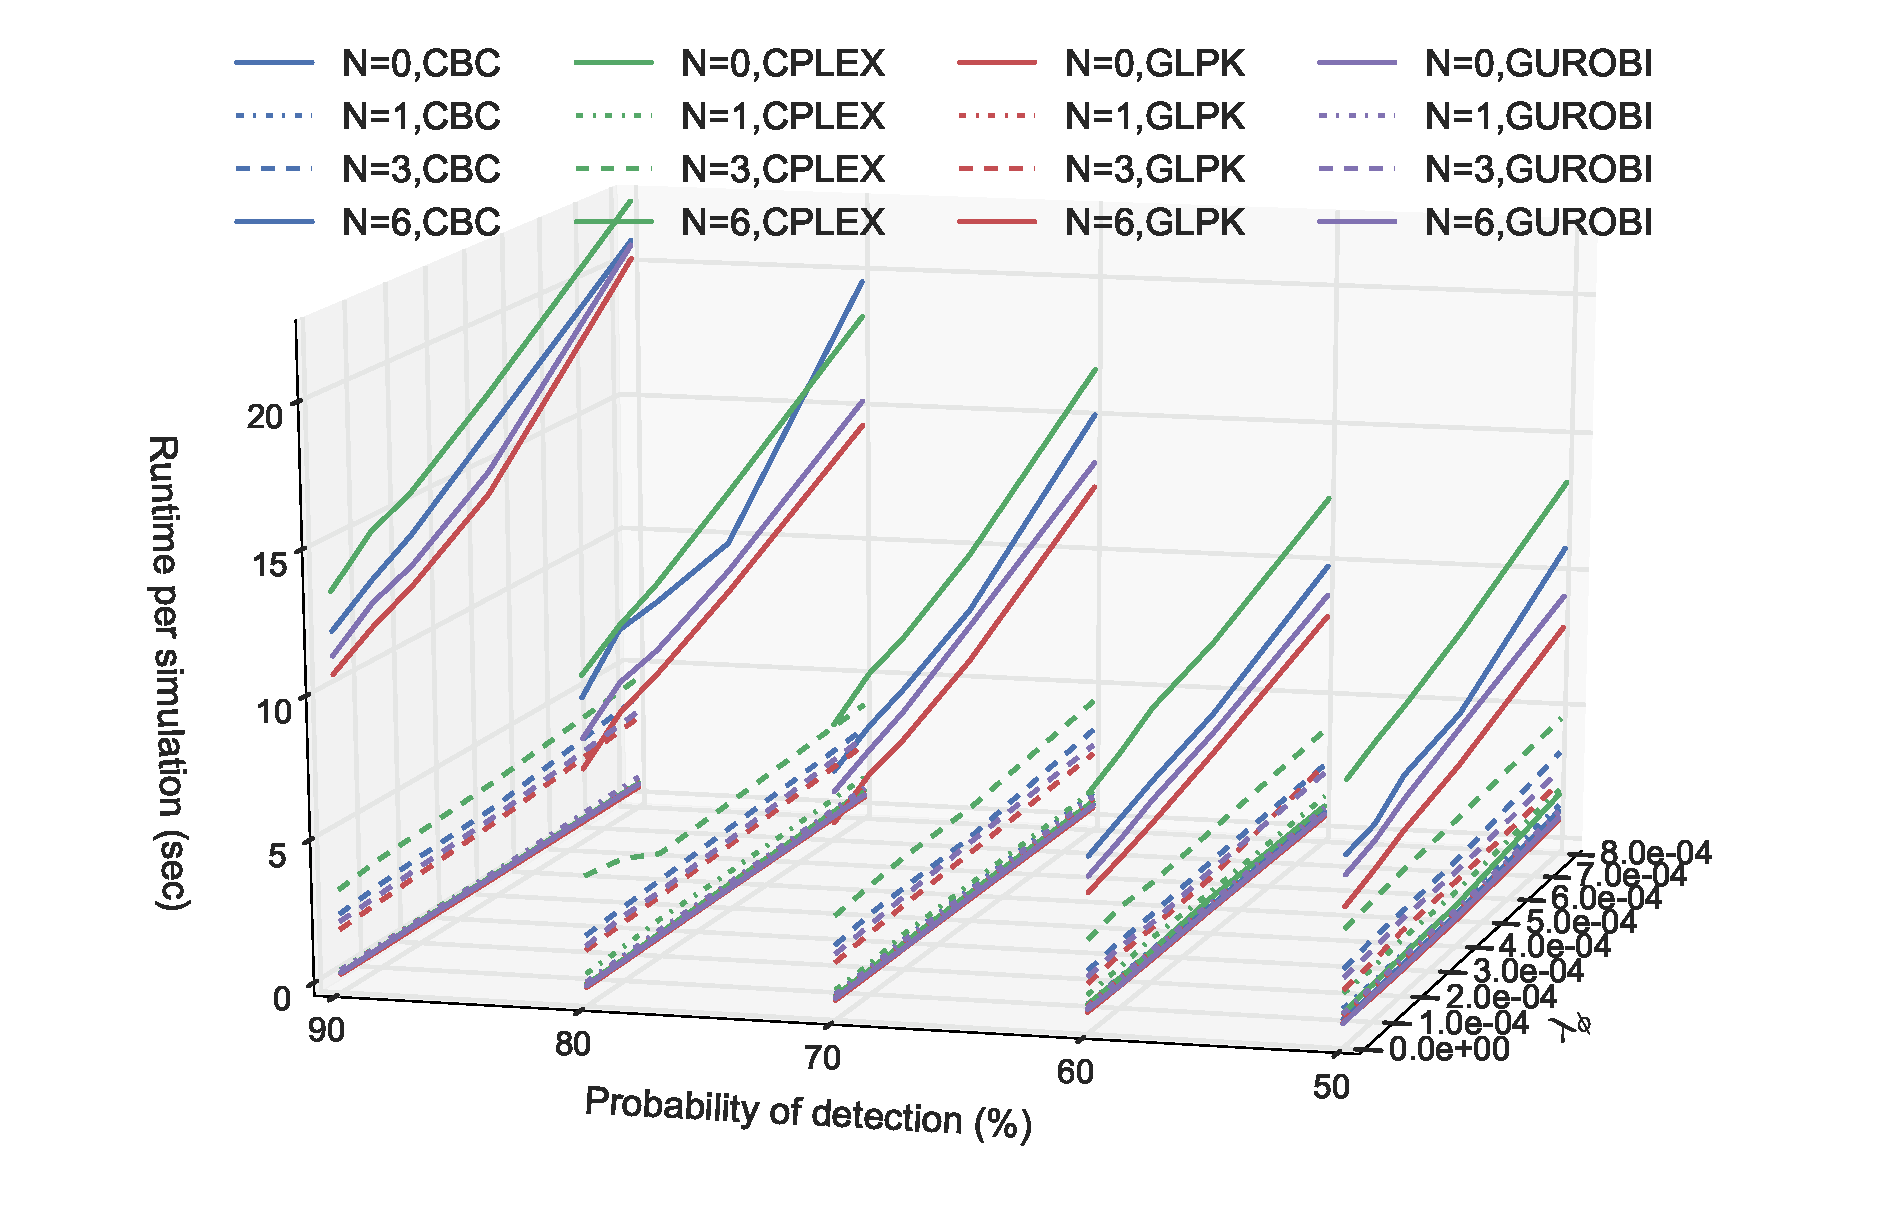
\includegraphics[clip, trim=0cm 1.5cm 0cm 0cm,width=\textwidth]{dynamic_and_static_agents_narrow_space_cropped_runtime}
\caption{Runtime for scenario 4}
\label{fig:runtime_scenario_4}
\end{figure}

\begin{figure}[H]
\centering
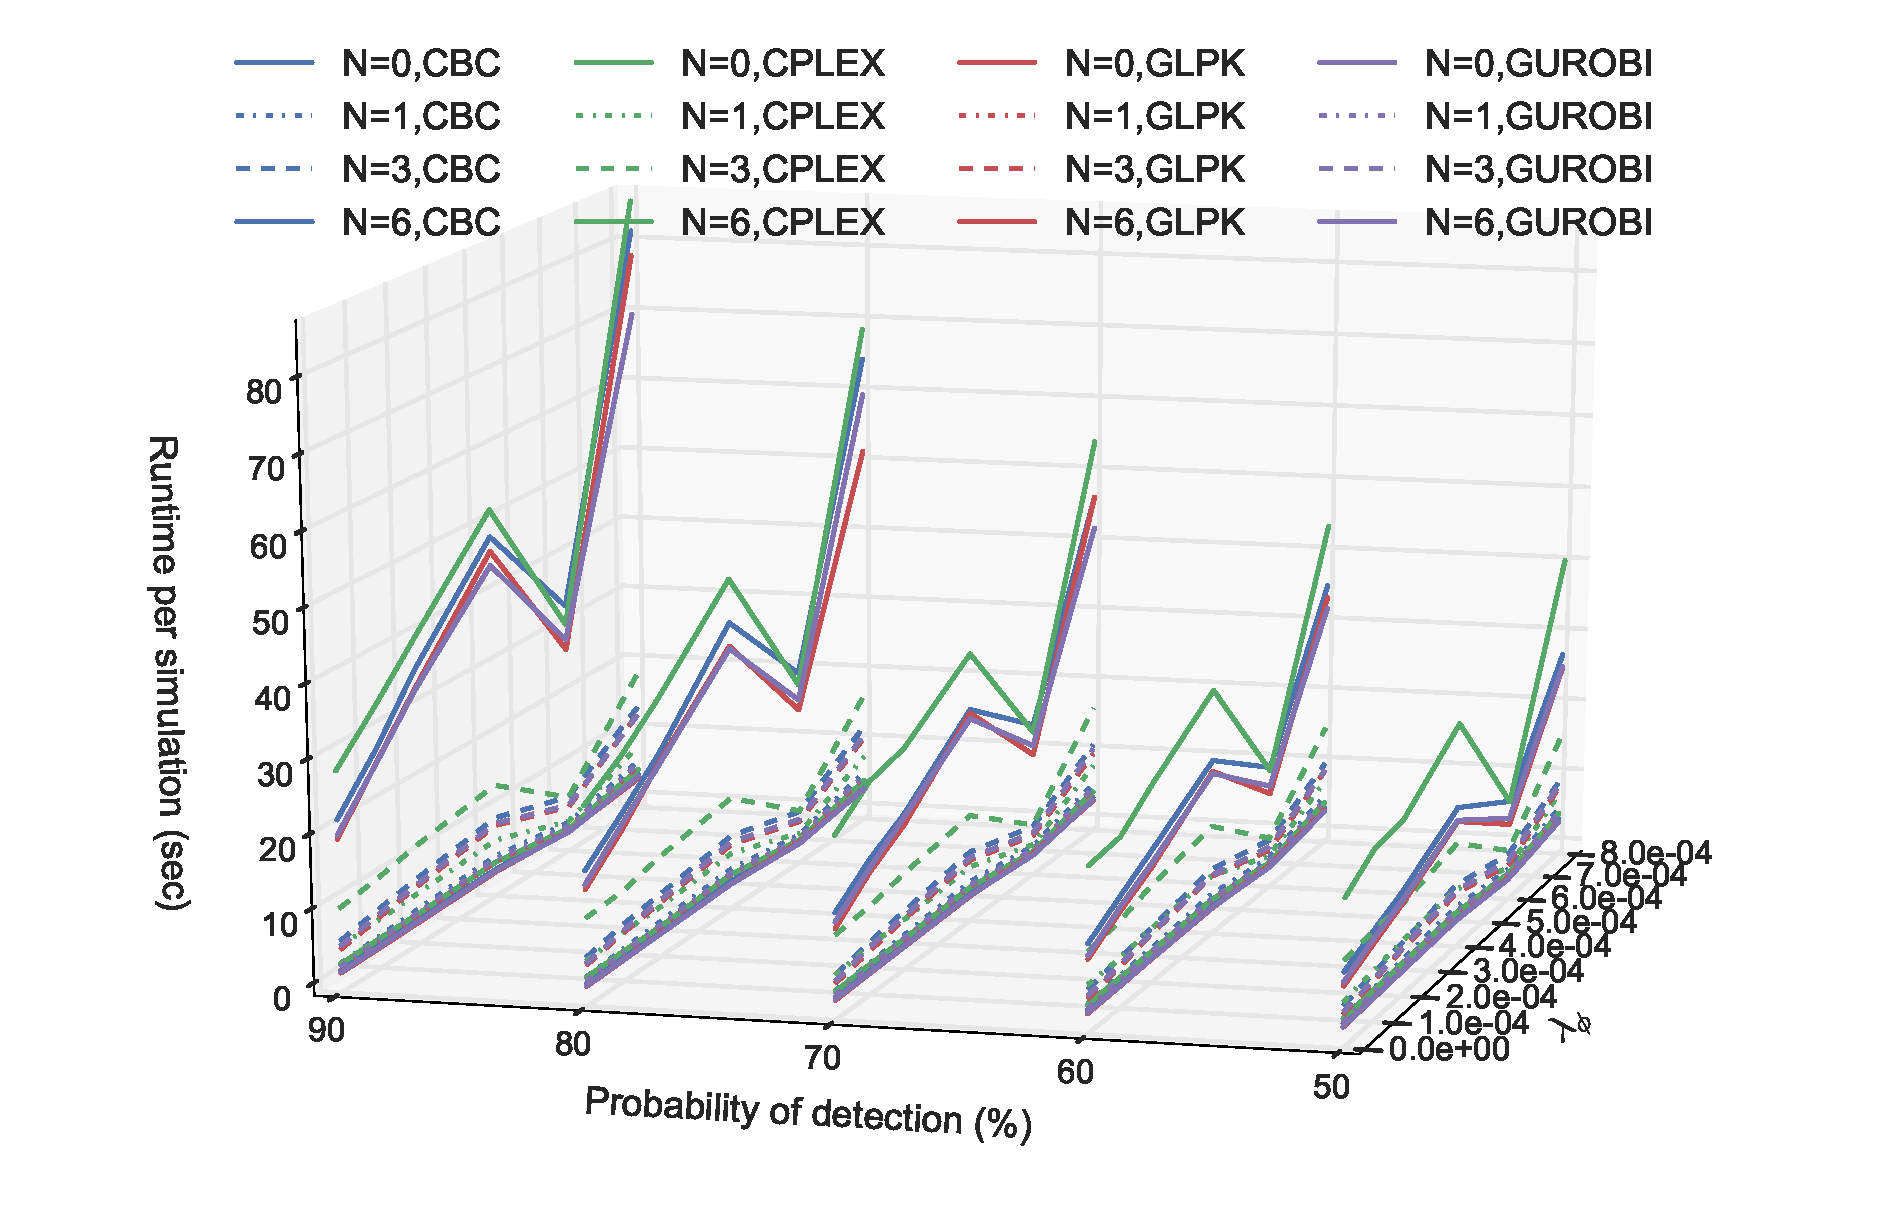
\includegraphics[clip, trim=0cm 1.5cm 0cm 0cm,width=\textwidth]{parallel_targets_1hz_runtime}
\caption{Runtime for scenario 5}
\label{fig:runtime_scenario_5}
\end{figure}

\begin{figure}[H]
\centering
\includegraphics[clip, trim=0cm 1.5cm 0cm 0cm,width=\textwidth]{{parallel_targets_0.5hz_runtime}.pdf}
\caption{Runtime for scenario 6}
\label{fig:runtime_scenario_6}
\end{figure}

\subsection{Track loss performance}
From the simulation results in Figure \ref{fig:dynamic_agents_full_cooperation_cropped} to \ref{fig:parallel_targets_1hz} in the appendix, it can be observed that the different solvers perform practically identically when it comes to track performance. From Figure \ref{fig:tracking_performance}, it can be seen that the number of lost tracks is proportional to the clutter level at an inverse proportional rate to the probability of detection $P_D$. An interesting observation is the return on investment regarding the number of scans to evaluate (N-scan). For instance, with $P_D=0.7$ the difference between $N=3$ and $N=6$ is marginal, at least when the clutter level is within reasonable levels ($\lambda_\phi < 4 \cdot 10^{-4}$). With $P_D=0.5$ is can be seen that the pay-off is much higher for the extra computational cost with 15\% improvement between $N=3$ and $N=6$.

Scenario 1-4 was simulated within a very small area where the targets had good separation both at the start and at the end of the simulation. This gives the algorithm more \glspl{scan} to figure out the correct association, after any multi-target conflicts that could arise when tracks are close to each other, and hence gives better track loss figures. In scenario 5-6 the targets start off spatially much closer and are moving faster. This leads to a situation more vulnerable to misdetections, and is an example of a situation where a high $N$-scan is beneficial.

\subsection{Time performance}
From Figure \ref{fig:runtime_scenario_1} to \ref{fig:runtime_scenario_6} it can be seen that the solvers have similar execution times, though with a very consistent difference in scenario 1 to 4. In these scenarios the \gls{glpk} solver is the fastest with 5-10 seconds compared with the slowest in these scenarios, \gls{cplex}. This trend is most likely caused by the different amount of overhead in the solvers, where IBM's \gls{cplex}, which is marked leading in many ways, might have way more initialization and setup procedures compared GNU's \gls{glpk}. In scenario 5 and 6, a different and more varying trend is visible. Here we see that both \gls{gurobi} and \gls{glpk} are fastest in different situations, and generally all other solvers than \gls{cplex} perform quite similar.

The run time increases linearly with the amount of clutter, which is expected as most of the operations run in the algorithm are based on tree operations with $O(E+V)$ run time. The structure in a track-tree implies that each vertex has one edge, hence any \gls{dfs} based operations will have run time  $O(2V)=O(V)$. The run time increases exponentially with the size of N, which is natural since the number of hypotheses that must be considered is exponentially larger.

\subsubsection{Bottle necks}
To study the effect parallel computation have on the tree growing task, a selected scan processing runtime was recorded with different amount of \gls{cpu} cores. Table \ref{tab:runtime_parallel} compares the run time averaged over 10 runs for the same scan, with different amount of parallel processes on a 4 core computer.

\begin{table}
\centering
\begin{tabular}{c c c c c c}
\bfseries Processes & \bfseries Total & \bfseries Grow & \bfseries Cluster & \bfseries Optimize & \bfseries Prune \\ \hline
\csvreader[head to column names]{{data/parallelTimeLog_ITK.csv}}{}
{\Processes & \Total & \Grow & \Cluster & \Optimize & \Prune \\\hline}
\end{tabular}
\caption{Runtime of a scan with different amount of processes (time in ms)}	
\label{tab:runtime_parallel}
\end{table}

Since the growing task is the only part of the algorithm that is utilizing on multiple cores, it is the only task that changes significantly. The multi processing of the growing task is implemented in a master-worker configuration, where the task is divided into $n-1$ equal chunks running on $n-1$ cores with the main process handling all the "worker" processes.  The run time increases when going from one to two processes, which is expected since the entire job is copied to another process, processed, and copied back. With any further increase in processor count, the execution time is expected to decline, which is also the case. At a certain core count, the time used to splitting up the task, distribute it to all the cores and collecting their results will become larger than the benefit of faster computation in each core. At this point, the overhead of parallizing the work leads to starvation of the workers and increased total run-time. On the four core machine, this limit is not reached, but by looking at Table \ref{tab:runtime_parallel_aws} in the appendix, displaying the runtime of the same program on a server with virtual \glspl{cpu}, it can be seen that the fastest execution time is with 6 cores. The scaling per core is worse on the virtualized server, possibly because the overhead of moving data to and forth the cores is larger. This means that running on a dedicated \gls{cpu} with more than four cores could yield higher optimal core count and thus better runtime performance. 


From Table \ref{tab:runtime_parallel_percentage}, we can see that the tree growing task is responsible for about one quarter of the run-time for this particular scan. Further analysis of the tree growing reveals that the creation of new nodes are the main contributor to the run time, with $97-98\%$ of the growing task.
\begin{table}
\centering
\begin{tabular}{c c c c c}
\bfseries Processes & \bfseries Grow & \bfseries Cluster & \bfseries Optimize & \bfseries Prune \\ \hline
\csvreader[head to column names,respect percent=true]{{data/parallelTimeLogPercentage_ITK.csv}}{}
{\Processes & \Grow \% & \Cluster \% & \Optimize \% & \Prune \% \\\hline }
\end{tabular}
\caption{Runtime distribution percentage}	
\label{tab:runtime_parallel_percentage}
\end{table}

\begin{table}
\centering
\begin{tabular}{c c c c c}
\bfseries Processes & \bfseries Search & \bfseries Predict & \bfseries Create & \bfseries Add \\ \hline
\csvreader[head to column names,respect percent=true]{{data/parallelTimeLogDistribution_ITK.csv}}{}
{\Processes & \Search \% & \Predict \% & \Create \% & \Add \% \\\hline }
\end{tabular}
\caption{Worker runtime distribution percentage}	
\label{tab:worker_parallel_percentage}
\end{table}